\lecture{4. The Covenant I Made With Their Fathers}{04}

\section{Introduction}

\begin{frame}
\frametitle{Commitments can be scary}
\begin{center}

\includegraphics[trim = 1.5in .5in 1.5in .5in, clip=true, height=0.8\textheight]{figures/ballAndChain.jpg}
\end{center}
\note{09:30}
\note[item]{We don't like responsibility}
\end{frame}

\begin{frame}
\frametitle{God wants a relationship with people}
\framesubtitle{Jeremiah 31:31-34}
	\keyversehiglight{they shall be my people}

\note{09:32}
\note[item]{The last two weeks were `I will be their God, they shall be my people'}
\note[item]{These phrases are themes throughout the bible}
\note[item]{These phrases are relationship focused}
\note[item]{This week we will discuss the fact that relationships come with a responsibility.}
\note[item]{We're going to strike Lesson 7}
\end{frame}

\begin{goals}
\goal Examine the role that covenants play in God's relationship with man
\goal Establish the importance of faith in both the Old and New Covenants
\goal Reflect on any ways that Christians could `return' to the weaknesses of Old Covenant
\end{goals}

\section{The importance of covenants}

\begin{frame}
\frametitle{Covenants of God through time}
\framesubtitle{}
\begin{columns}[T]
\begin{column}{0.4\textwidth}
	`covenant' (ESV)
	\begin{center}
	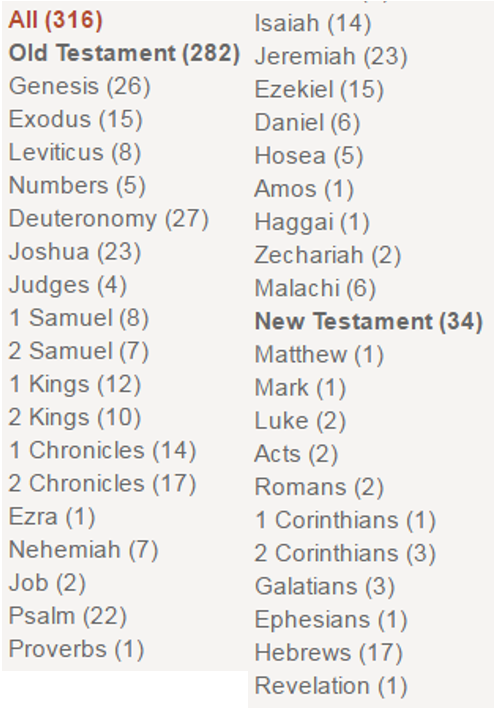
\includegraphics[width=\columnwidth]{figures/covenant.png}
		\end{center}
	{\footnotesize $-42$ `ark of the covenant'}
\end{column}
\begin{column}{0.6\textwidth}
	\begin{itemize}
	\item{Noah}
	\item{Abraham}
	\item{Isaac}
	\item{Jacob}
	\item{Children of Israel}
	\item{David}
	\end{itemize}
\end{column}
\end{columns}

\note{09:35}
\end{frame}

\begin{frame}
\frametitle{Covenants require collateral}
% image collateral
\note{09:38}
\end{frame}

\begin{frame}
\note{Covenants have responsibilities on both side}

\end{frame}
\begin{frame}
\frametitle{The `Old' Covenant}

\note{09:38}
\note[item] AKA The Law of Moses
\end{frame}

\begin{frame}
\frametitle{The Old Covenant had weaknesses}

\note{09:42}
\end{frame}

\section{The importance of faith}

\begin{frame}
\frametitle{The Old Covenant required faith}

\note{09:44}
\note[item]{This seems to contradict Galatians 3:12}
\note[item]{Paul is talking about how people tried to \emph{keep} the Law, not the weakness of the Law itself}
\end{frame}

\begin{frame}
\frametitle{The Law is both a thing and an idea}

\note{09:46}
\note[item]{People try to shoehorn every instance of the word `law' into meaning simply the Law of Moses.}
\note[item]{Why do they do that? Because there are many, so called `Christians' who would say that you don't have to do good works to go to heaven.}
\note[item]{These people understand any passages that say `law' incorrectly to mean that `any' attempt to do good works is futile and has no bearing on whether or not you enter heaven.}
\note[item]{That's a misunderstanding}
\note[item]{So, to combat that, we say, `Well, these passages are talking about the Law of Moses, not just doing good works in general'.}
\note[item]{And, we're correct in saying that.}
\note[item]{Unfortunately, what happens when we treat the word `law' as simply the Law of Moses, we are taking large chunks of the New Testament and saying, ``That doesn't apply to me.''}
\note[item]{The entire books of Galatians and Romans}
\note[item]{The term `law' is bigger than simply the Law of Moses.}
\note[item]{We'll talk more about this, in `I will write my law on their hearts'}
\note[item]{So I need to set the stage here.}
\end{frame}

\begin{frame}
\frametitle{}
\framesubtitle{}
\begin{center}
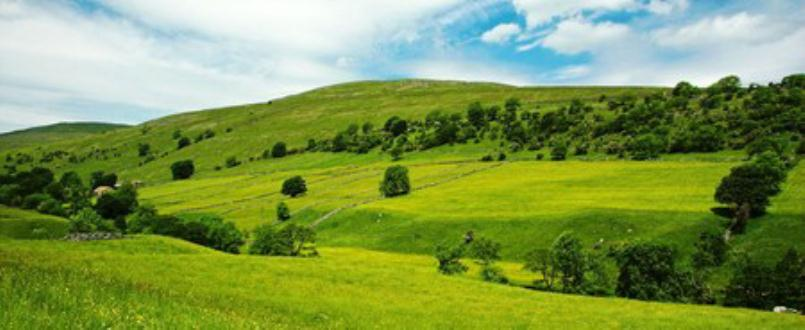
\includegraphics[width=0.8\textwidth]{figures/land.jpg}
\end{center}
\begin{itemize}
\item ``I will \ldots bring them to their own land.''
\item ``Make them one nation''
\item ``One king''
\item ``My dwelling place shall be with them''
\item ``I will be their God and they shall be my people''
\end{itemize}

\note{09:50}
\note[item]{The people of God always have a land, a place, a possession.}
\note[item]{The prophecy must refer to spiritual Israel, because restoration of the physical Northern tribes never did occur.}
\note[item]{With all this emphasis on the land, it's no wonder that the people of Israel had a hard time accepting Jesus, and why the physical restoration of Israel is a key doctrine for premellinialists.}
\note[item]{They were thinking that God had forgotten them.}
\note[item]{That times would never get better.}
\end{frame}

\begin{frame}
\frametitle{God's people still have a promised land}
\framesubtitle{Hebrews 11:13-16}
13 These all died in faith, not having received the things promised, but having seen them and greeted them from afar, and having acknowledged that they were strangers and exiles on the earth. 14 For people who speak thus make it clear that they are seeking a homeland. 15 If they had been thinking of that land from which they had gone out, they would have had opportunity to return. 16 But as it is, they desire a better country, that is, a heavenly one. Therefore God is not ashamed to be called their God, for he has prepared for them a city.

\note{09:54}
\note[item]{Yes, Abraham was promised a physical land, but it was also a spiritual land.}
\note[item]{The faithful from times past looked forward to the spiritual land, not the physical land.}
\note[item]{We have that same promised land -- entrance into the kingdom of God, and, ultimately, heaven}
\end{frame}

\section{Don't return to the Old Covenant6}

\begin{frame}
\frametitle{The Lord made Israel special}
\framesubtitle{Deut. 10:12-22}
\begin{columns}[T]
\begin{column}{0.5\textwidth}
\begin{center}

\includegraphics[width=\columnwidth]{figures/uniqueFish.jpg}
\end{center}
\end{column}
\begin{column}{0.5\textwidth}
\begin{itemize}
\item No one else got the benefits that Israel did.
\item No one else had the requirements that Israel did.
\end{itemize}
\end{column}
\end{columns}

\note{09:56}
\note[item]{Same verse quoted in Luke 10 last week about loving the Lord}
\note[item]{God selected you above all peoples.  As a result, serve Him.}
\end{frame}

\begin{frame}
	\frametitle{The Lord made Christians special}
	\framesubtitle{I Peter 2:9-10}
	\begin{columns}[T]
	\begin{column}{0.5\textwidth}
		\begin{center}
		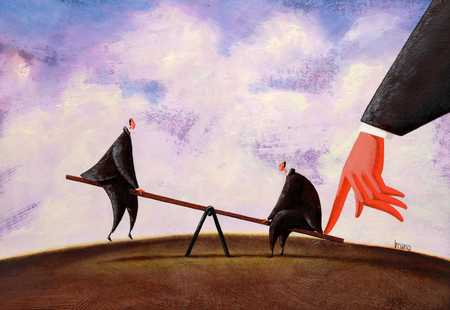
\includegraphics[width=\columnwidth]{figures/unfairAdvantage.jpg}
		\end{center}
	\end{column}
	\begin{column}{0.5\textwidth}
		\begin{itemize}
		\item We are a chosen race (like Israel).
		\item We are a royal priesthood (like Judah and Levi put together!).
		\end{itemize}
	\end{column}
	\end{columns}
	
\note{09:58}
\note[item]{The Israelites were chosen first}
\note[item]{We weren't a people until God gave us the opportunity.}
\note[item]{Investment bankers usually come from rich families.}
\note[item]{Starting out wealthy has its advantages}
\note[item]{This passage reminds us that we're the privileged ones.}
\end{frame}

\begin{frame}
\frametitle{God adopts us as sons}
\framesubtitle{Romans 8:12-17}
\begin{columns}[T]
\begin{column}{0.5\textwidth}
	
\includegraphics[width=\columnwidth]{figures/toddAndEzra.jpg}
\end{column}
\begin{column}{0.5\textwidth}
	\begin{itemize}
	\item ``Abba, Father'' reveals the closeness we have with God.
	\item We are heirs with Christ.
	\item We will be glorified with Christ.
	\end{itemize}
\end{column}
\end{columns}

\note{10:00}
\note[item]{You look at that picture and think, `Ah, cute'}
\note[item]{I look at that picture and see something completely different -- My son}
\note[item]{That's what `Abba, Father' means}
\note[item]{\emph{What are we heirs of?}  The everlasting kingdom prophesied in Ezekiel 37.}
\note[item]{Some of those blessings we receive now (\emph{e.g.}, entrance into the kingdom)}
\note[item]{Some of those blessings are yet to be revealed (\emph{e.g.}, resurrection from the dead).}
\end{frame}

\begin{frame}
\frametitle{The Lord is with His people from start to finish}
\framesubtitle{Romans 8:28-30}
\begin{columns}[T]
\begin{column}{0.4\textwidth}
	\begin{center}
	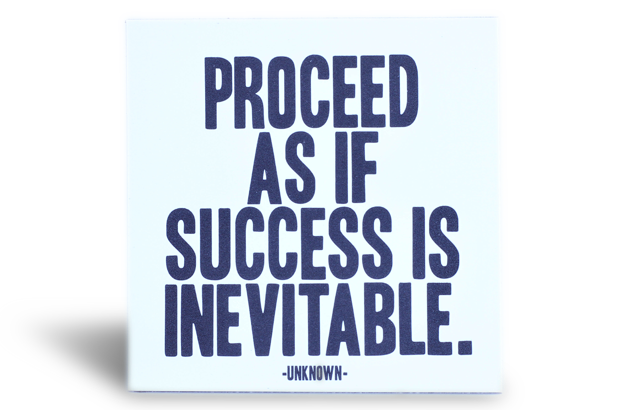
\includegraphics[width=1.3\columnwidth]{figures/success.png}
	\end{center}
\end{column}
\begin{column}{0.6\textwidth}
\begin{itemize}
	\item This passage should encourage us, not simply generate theological discussions.
	\item God's preparations for His people started before time.
	\item God's support of His people will continue through the end of time. 
\end{itemize}
\end{column}
\end{columns}

\note{10:05}	
\note[item]{\emph{Below is a prepared answer if I'm asked about predestination}}
\note[item]{Calvinists misunderstand the sovereignty of God.}
\note[item]{I have no issue with God knowing what happens in the future or even knowing ahead of time those who will be lost or saved.}
\note[item]{God knew ahead of time the poor decisions people would make and what the outcome of those decisions would be (\emph{e.g.}, Rom. 9, Esau, Pharaoh, Judas, Peter).}
\note[item]{Foreknowledge is not causation, however.}
\note[item]{God does not `select' people apart from their own decisions}
\note[item]{Calvinists assume that our decisions are \emph{totally} driven by either our sinful human nature (over which we have no control) or the miraculous influence of the Holy Spirit (for salvation).}
%\note[item]{Sociologists have the same problem.  Their whole field  is predicated on the assumption that your environment is the sole determinants of your choices.}
\note[item]{This contradicts Matt 22, which we've already discussed.}	
\end{frame}

\section{Review}

\begin{frame}
\frametitle{They shall be my people}
	\begin{itemize}
		\item God wants volunteers
		\item God makes a way for His people
		\item God gives His people eternal possessions
		\item God's people are special
		\item The best days are still ahead of us
	\end{itemize}

\note{10:10}
\note[item]{You are special.}
\note[item]{Act like it.}
\note[item]{Better days are ahead, because you are God's people.}
\end{frame}
